\chapter{Combinatòria}

\index{combinatòria}

La \key{combinatòria} estudia mètodes per comptar combinacions
d'objectes. Normalment, l'objectiu és trobar una manera de comptar les
combinacions de manera eficient sense generar cada combinació per
separat.

Per exemple, considereu el problema de comptar el nombre de maneres de
representar un nombre enter $n$ com a suma de nombres enters
positius. Per exemple, hi ha 8 representacions per $4$:
\begin{multicols}{2}
\begin{itemize}
\item $1+1+1+1$
\item $1+1+2$
\item $1+2+1$
\item $2+1+1$
\item $2+2$
\item $3+1$
\item $1+3$
\item $4$
\end{itemize}
\end{multicols}


Sovint, un problema combinatori es pot resoldre mitjançant una funció
recursiva. En aquest problema, podem definir una funció $f(n)$ que
dóna el nombre de representacions de $n$. Per exemple, $f(4)=8$ segons
l'exemple anterior. Els valors de la funció es poden calcular
recursivament de la següent manera:
\begin{equation*}
    f(n) = \begin{cases}
               1               & n = 0\\
               f(0)+f(1)+\cdots+f(n-1) & n > 0\\
           \end{cases}
\end{equation*}
El cas base és $f(0)=1$, perquè la suma buida representa el nombre
0. Aleshores, si $n>0$, considerem totes les maneres d'escollir el
primer nombre de la suma. Si el primer nombre és $k$, hi ha $f(n-k)$
representacions per a la part restant de la suma. Així, calculem la
suma de tots els valors de la forma $f(n-k)$ on $k<n$.

Els primers valors de la funció són:
\[
\begin{array}{lcl}
f(0) & = & 1 \\
f(1) & = & 1 \\
f(2) & = & 2 \\
f(3) & = & 4 \\
f(4) & = & 8 \\
\end{array}
\]


De vegades, una fórmula recursiva es pot substituir per una fórmula de
forma tancada. En aquest problema,
\[
f(n)=2^{n-1},
\]
que es basa en el fet que hi ha $n-1$ posicions possibles per als
signes + a la suma i podem triar-ne qualsevol subconjunt.

\section{Coeficients binomials}

\index{coeficient binomial}

El \key{coeficient binomial} ${n \choose k}$ és igual al nombre de
maneres de triar un subconjunt de $k$ elements d'un conjunt de $n$
elements. Per exemple, ${5 \choose 3}=10$, perquè el conjunt
$\{1,2,3,4,5\}$ té 10 subconjunts de 3 elements: \[ \{1,2,3\} ,
\{1,2,4\}, \{1,2,5\}, \{1,3,4\}, \{1,3,5\}, \{1,4,5\} , \{2,3,4\},
\{2,3,5\}, \{2,4,5\}, \{3,4,5\} \]

\subsubsection{Fórmula 1}

Els coeficients binomials es poden calcular recursivament de la
següent manera:

\[
{n \choose k}  =  {n-1 \choose k-1} + {n-1 \choose k}
\]

La idea és fixar un element $x$ al conjunt. Si $x$ s'inclou al
subconjunt, hem de triar $k-1$ elements d'entre $n-1$ elements, i si
$x$ no s'inclou al subconjunt, hem de triar $k$ elements de $n-1$
elements.

Els casos base de la recursivitat són
\[
{n \choose 0}  =  {n \choose n} = 1,
\]
perquè sempre hi ha exactament una manera de construir un subconjunt
buit i un subconjunt que conté tots els elements.

\subsubsection{Fórmula 2}

Una altra manera de calcular els coeficients binomials és:
\[
{n \choose k}  =  \frac{n!}{k!(n-k)!}.
\]


Hi ha $n!$ permutacions de $n$ elements. Passem per totes les
permutacions i sempre incloem els primers $k$ elements de la
permutació al subconjunt. Com que l'ordre dels elements dintre i fora
del subconjunt no importa, el resultat es divideix per $k!$ i
$(n-k)!$

\subsubsection{Propietats}

Per als coeficients binomials,
\[
{n \choose k}  =  {n \choose n-k},
\]
perquè en realitat dividim un conjunt de $n$ elements en dos
subconjunts: el primer conté $k$ elements i el segon conté $n-k$
elements.

La suma dels coeficients binomials és
\[
{n \choose 0}+{n \choose 1}+{n \choose 2}+\ldots+{n \choose n}=2^n.
\]

La raó del nom ''coeficient binomial'' es pot veure quan elevem el binomi
$(a+b)$ a la potència $n$-èsima:

\[ (a+b)^n = {n \choose 0} a^nb^0 + {n \choose 1} a^{n-1} b^1 + \ldots + {n \choose n-1} a^1 b^{n-1} + {n \choose n} a^0 b^n. \]

\index{Triangle de Pascal}

Els coeficients binomials també apareixen al \key{triangle de Pascal},
on cada valor és igual a la suma dels dos valors anteriors:
\begin{center}
\begin{tikzpicture}{0.9}
\node at (0,0) {1};
\node at (-0.5,-0.5) {1};
\node at (0.5,-0.5) {1};
\node at (-1,-1) {1};
\node at (0,-1) {2};
\node at (1,-1) {1};
\node at (-1.5,-1.5) {1};
\node at (-0.5,-1.5) {3};
\node at (0.5,-1.5) {3};
\node at (1.5,-1.5) {1};
\node at (-2,-2) {1};
\node at (-1,-2) {4};
\node at (0,-2) {6};
\node at (1,-2) {4};
\node at (2,-2) {1};
\node at (-2,-2.5) {$\ldots$};
\node at (-1,-2.5) {$\ldots$};
\node at (0,-2.5) {$\ldots$};
\node at (1,-2.5) {$\ldots$};
\node at (2,-2.5) {$\ldots$};
\end{tikzpicture}
\end{center}


\subsubsection{Caixes i boles}

''Caixes i boles'' és un model útil, on comptem les maneres de
col·locar $k$ boles en $n$ caixes. Considerem tres escenaris:

\textit{Escenari 1}: cada caixa pot contenir com a màxim una bola. Per
exemple, quan $n=5$ i $k=2$, hi ha 10 solucions:


\begin{center}
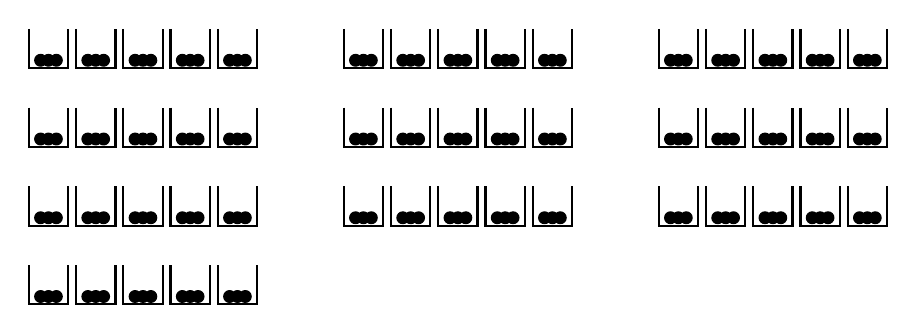
\begin{tikzpicture}[scale=0.5]
\newcommand\lax[3]{
\path[draw,thick,-] (#1-0.5,#2+0.5) -- (#1-0.5,#2-0.5) --
                    (#1+0.5,#2-0.5) -- (#1+0.5,#2+0.5);
\ifthenelse{\equal{#3}{1}}{\draw[fill=black] (#1,#2-0.3) circle (0.15);}{}
\ifthenelse{\equal{#3}{2}}{\draw[fill=black] (#1-0.2,#2-0.3) circle (0.15);}{}
\ifthenelse{\equal{#3}{2}}{\draw[fill=black] (#1+0.2,#2-0.3) circle (0.15);}{}
}
\newcommand\laa[7]{
    \lax{#1}{#2}{#3}
    \lax{#1+1.2}{#2}{#4}
    \lax{#1+2.4}{#2}{#5}
    \lax{#1+3.6}{#2}{#6}
    \lax{#1+4.8}{#2}{#7}
}

\laa{0}{0}{1}{1}{0}{0}{0}
\laa{0}{-2}{1}{0}{1}{0}{0}
\laa{0}{-4}{1}{0}{0}{1}{0}
\laa{0}{-6}{1}{0}{0}{0}{1}
\laa{8}{0}{0}{1}{1}{0}{0}
\laa{8}{-2}{0}{1}{0}{1}{0}
\laa{8}{-4}{0}{1}{0}{0}{1}
\laa{16}{0}{0}{0}{1}{1}{0}
\laa{16}{-2}{0}{0}{1}{0}{1}
\laa{16}{-4}{0}{0}{0}{1}{1}

\end{tikzpicture}
\end{center}


En aquest escenari, la resposta és directament el coeficient binomial
${n \choose k}$.

\textit{Escenari 2}: una caixa pot contenir diverses boles. Per exemple, quan $n=5$ i $k=2$, hi ha 15 solucions:


\begin{center}
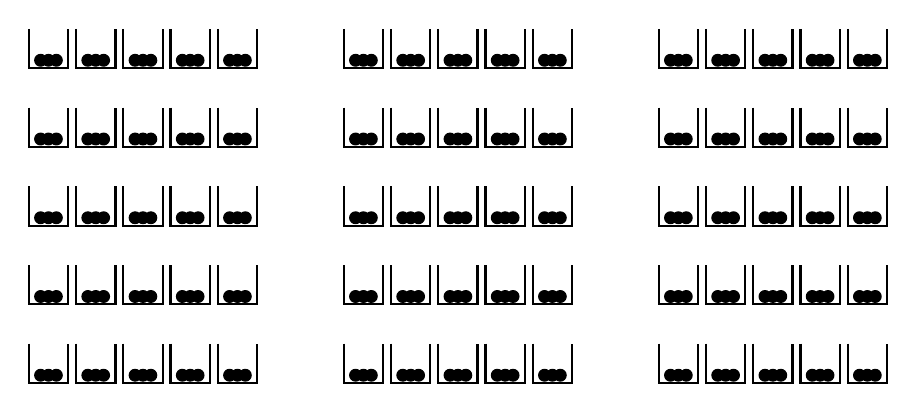
\begin{tikzpicture}[scale=0.5]
\newcommand\lax[3]{
\path[draw,thick,-] (#1-0.5,#2+0.5) -- (#1-0.5,#2-0.5) --
                    (#1+0.5,#2-0.5) -- (#1+0.5,#2+0.5);
\ifthenelse{\equal{#3}{1}}{\draw[fill=black] (#1,#2-0.3) circle (0.15);}{}
\ifthenelse{\equal{#3}{2}}{\draw[fill=black] (#1-0.2,#2-0.3) circle (0.15);}{}
\ifthenelse{\equal{#3}{2}}{\draw[fill=black] (#1+0.2,#2-0.3) circle (0.15);}{}
}
\newcommand\laa[7]{
    \lax{#1}{#2}{#3}
    \lax{#1+1.2}{#2}{#4}
    \lax{#1+2.4}{#2}{#5}
    \lax{#1+3.6}{#2}{#6}
    \lax{#1+4.8}{#2}{#7}
}

\laa{0}{0}{2}{0}{0}{0}{0}
\laa{0}{-2}{1}{1}{0}{0}{0}
\laa{0}{-4}{1}{0}{1}{0}{0}
\laa{0}{-6}{1}{0}{0}{1}{0}
\laa{0}{-8}{1}{0}{0}{0}{1}
\laa{8}{0}{0}{2}{0}{0}{0}
\laa{8}{-2}{0}{1}{1}{0}{0}
\laa{8}{-4}{0}{1}{0}{1}{0}
\laa{8}{-6}{0}{1}{0}{0}{1}
\laa{8}{-8}{0}{0}{2}{0}{0}
\laa{16}{0}{0}{0}{1}{1}{0}
\laa{16}{-2}{0}{0}{1}{0}{1}
\laa{16}{-4}{0}{0}{0}{2}{0}
\laa{16}{-6}{0}{0}{0}{1}{1}
\laa{16}{-8}{0}{0}{0}{0}{2}

\end{tikzpicture}
\end{center}


El procés de col·locació de les boles a les caixes es pot representar
com una cadena amb els símbols ''o'' i ''$\rightarrow$''. Inicialment,
suposem que estem a la casella més a l'esquerra. El símbol ''o''
significa que col·loquem una bola a la casella actual, i el símbol
''$\rightarrow$'' significa que ens movem a la casella següent a la
dreta.

Amb aquesta notació, cada solució és una cadena que conté $k$ vegades
el símbol ''o'' i $n-1$ vegades el símbol ''$\rightarrow$''. Per
exemple, la solució superior dreta de la imatge de dalt correspon a la
cadena ''$\rightarrow$ $\rightarrow$ o $\rightarrow$ o
$\rightarrow$''. Així, el nombre de solucions és ${k+n-1 \choose k}$.

\textit{Escenari 3}: Cada caixa pot contenir com a màxim una bola i, a
més, no permetem que dues caixes adjacents continguin ambdues una bola. Per
exemple, quan $n=5$ i $k=2$, hi ha 6 solucions:




\begin{center}
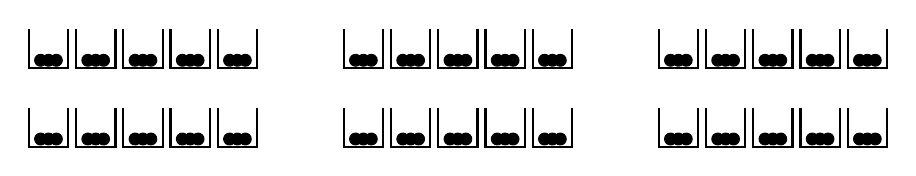
\begin{tikzpicture}[scale=0.5]
\newcommand\lax[3]{
\path[draw,thick,-] (#1-0.5,#2+0.5) -- (#1-0.5,#2-0.5) --
                    (#1+0.5,#2-0.5) -- (#1+0.5,#2+0.5);
\ifthenelse{\equal{#3}{1}}{\draw[fill=black] (#1,#2-0.3) circle (0.15);}{}
\ifthenelse{\equal{#3}{2}}{\draw[fill=black] (#1-0.2,#2-0.3) circle (0.15);}{}
\ifthenelse{\equal{#3}{2}}{\draw[fill=black] (#1+0.2,#2-0.3) circle (0.15);}{}
}
\newcommand\laa[7]{
    \lax{#1}{#2}{#3}
    \lax{#1+1.2}{#2}{#4}
    \lax{#1+2.4}{#2}{#5}
    \lax{#1+3.6}{#2}{#6}
    \lax{#1+4.8}{#2}{#7}
}

\laa{0}{0}{1}{0}{1}{0}{0}
\laa{0}{-2}{1}{0}{0}{1}{0}
\laa{8}{0}{1}{0}{0}{0}{1}
\laa{8}{-2}{0}{1}{0}{1}{0}
\laa{16}{0}{0}{1}{0}{0}{1}
\laa{16}{-2}{0}{0}{1}{0}{1}
\end{tikzpicture}
\end{center}


En aquest escenari, podem suposar que $k$ boles es col·loquen
inicialment en caixes i que hi ha una caixa buida entre dues caixes
adjacents. El que queda és triar les posicions de les caixes buides
restants. Hi ha $n-2k+1$ caixes d'aquest tipus i $k+1$ posicions per a
elles. Així, utilitzant la fórmula de l'escenari 2, el nombre de solucions
és ${n-k+1 \choose n-2k+1}$.

\subsubsection{Coeficients multinomials}

\index{coeficient multinomial}

El \key{coeficient multinomial}
\[ {n \choose k_1,k_2,\ldots,k_m} = \frac{n!}{k_1! k_2! \cdots k_m!}, \]
és el nombre de maneres en què podem dividir $n$ elements en
subconjunts de mides $k_1,k_2,\ldots,k_m$, on
$k_1+k_2+\cdots+k_m=n$. Els coeficients multinomials es poden veure
com una generalització dels coeficients binomials; si $m=2$, la
fórmula anterior correspon a la fórmula del coeficient binomial.

\section{Nombres de Catalan}

\index{Nombres de Catalan}

El \key{nombre de Catalan}\footnote{E. C. Catalan (1814--1894) va ser
un matemàtic belga.} $C_n$ és igual al nombre d'expressions de
parèntesis vàlides amb $n$ parèntesis esquerres i $n$ drets.

Per exemple, $C_3=5$, perquè podem construir les següents expressions
de parèntesis vàlides utilitzant tres parèntesis esquerres i drets:


\begin{itemize}[noitemsep]
\item \texttt{()()()}
\item \texttt{(())()}
\item \texttt{()(())}
\item \texttt{((()))}
\item \texttt{(()())}
\end{itemize}


\subsubsection{Expressions de parèntesis}

\index{expressió de parèntesis}

Què és exactament una \emph{expressió de parèntesis vàlida}? Les
regles següents defineixen amb precisió quines són les expressions
vàlides:


\begin{itemize}
\item L'expressió buida és vàlida.
\item Si l'expressió $A$ és vàlida,
l'expressió
\texttt{(}$A$\texttt{)} també és vàlida.
\item Si les expressions $A$ i $B$ són vàlides,
l'expressió $AB$ també ho és.
\end{itemize}


Una altra manera de caracteritzar les expressions de parèntesis
vàlides és que si triem qualsevol prefix d'aquesta expressió, ha de
contenir almenys tants parèntesis esquerre com parèntesis dret. A més,
l'expressió completa ha de contenir un nombre igual de parèntesis
esquerre i dret.

\subsubsection{Fórmula 1}

Els nombres de Catalan es poden calcular mitjançant la fórmula
\[ C_n = \sum_{i=0}^{n-1} C_{i} C_{n-i-1}.\]


La suma recorre les maneres de dividir l'expressió en dues parts de
manera que ambdues parts siguin expressions vàlides i la primera part
sigui tan curta com sigui possible, però no buida. Per a qualsevol
$i$, la primera part conté $i+1$ parells de parèntesis i el nombre
d'expressions és el producte dels valors següents:


\begin{itemize}
\item $C_{i}$: maneres de construir una expressió de parèntesis
  per la primera part, sense comptar els parentesis que envolten l'expressió.
\item $C_{n-i-1}$: maneres de construir una expressió de parèntesis
  per la segona part.
\end{itemize}

El cas base és $C_0=1$, perquè podem construir una expressió de
parèntesi buida fent servir zero parells de parèntesis.

\subsubsection{Fórmula 2}

Els nombres de Catalan també es poden calcular amb coeficients binomials:
\[ C_n = \frac{1}{n+1} {2n \choose n}\]
La fórmula es pot explicar de la següent manera:

Hi ha ${2n \choose n}$ maneres de construir una expressió de parèntesi
(no necessàriament vàlida) que conté $n$ parèntesis esquerre i $n$
parèntesis dret. Calculem el nombre d'expressions d'aquest tipus que
\emph{no} són vàlides.

Si una expressió de parèntesis no és vàlida, ha de contenir un prefix
on el nombre de parèntesis dret superi el nombre de parèntesis
esquerre. La idea és invertir cada parèntesi que pertany a aquest
prefix. Per exemple, l'expressió \texttt{())()(} conté un prefix
\texttt{())}, i després d'invertir el prefix, l'expressió es
converteix en \texttt{)((()(}).

L'expressió resultant consta de $n+1$ parèntesis esquerre i $n-1$
parèntesis dret. El nombre d'aquestes expressions és ${2n \choose
  n+1}$, que és igual al nombre d'expressions de parèntesis no
vàlides. Així, el nombre d'expressions de parèntesis vàlides es pot
calcular mitjançant la fórmula
\[{2n \choose n}-{2n \choose n+1} = {2n \choose n} - \frac{n}{n+1} {2n \choose n} = \frac{1}{n+1} {2n \choose n}.\]


\subsubsection{Comptar arbres}

Els nombres catalans també estan relacionats amb els arbres:

\begin{itemize}
\item hi ha $C_n$ arbres binaris de $n$ nodes
\item hi ha $C_{n-1}$ arbres arrelats de $n$ nodes
\end{itemize}
\noindent Per exemple, per a $C_3=5$, els arbres binaris són


\begin{center}
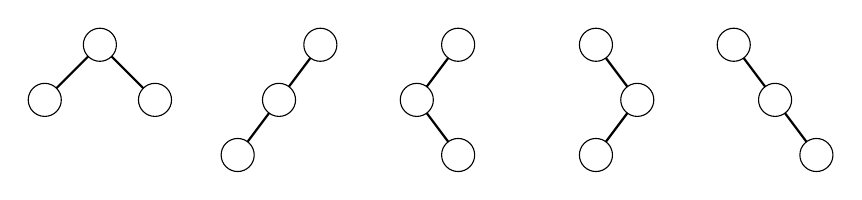
\begin{tikzpicture}[scale=0.7]
\path[draw,thick,-] (0,0) -- (-1,-1);
\path[draw,thick,-] (0,0) -- (1,-1);
\draw[fill=white] (0,0) circle (0.3);
\draw[fill=white] (-1,-1) circle (0.3);
\draw[fill=white] (1,-1) circle (0.3);

\path[draw,thick,-] (4,0) -- (4-0.75,-1) -- (4-1.5,-2);
\draw[fill=white] (4,0) circle (0.3);
\draw[fill=white] (4-0.75,-1) circle (0.3);
\draw[fill=white] (4-1.5,-2) circle (0.3);

\path[draw,thick,-] (6.5,0) -- (6.5-0.75,-1) -- (6.5-0,-2);
\draw[fill=white] (6.5,0) circle (0.3);
\draw[fill=white] (6.5-0.75,-1) circle (0.3);
\draw[fill=white] (6.5-0,-2) circle (0.3);

\path[draw,thick,-] (9,0) -- (9+0.75,-1) -- (9-0,-2);
\draw[fill=white] (9,0) circle (0.3);
\draw[fill=white] (9+0.75,-1) circle (0.3);
\draw[fill=white] (9-0,-2) circle (0.3);

\path[draw,thick,-] (11.5,0) -- (11.5+0.75,-1) -- (11.5+1.5,-2);
\draw[fill=white] (11.5,0) circle (0.3);
\draw[fill=white] (11.5+0.75,-1) circle (0.3);
\draw[fill=white] (11.5+1.5,-2) circle (0.3);
\end{tikzpicture}
\end{center}
i els arbres arrelats són
\begin{center}
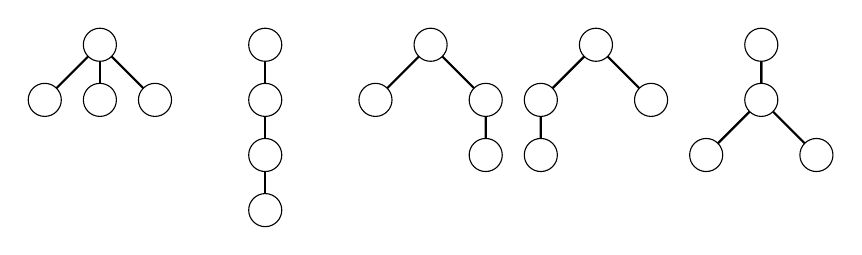
\begin{tikzpicture}[scale=0.7]
\path[draw,thick,-] (0,0) -- (-1,-1);
\path[draw,thick,-] (0,0) -- (0,-1);
\path[draw,thick,-] (0,0) -- (1,-1);
\draw[fill=white] (0,0) circle (0.3);
\draw[fill=white] (-1,-1) circle (0.3);
\draw[fill=white] (0,-1) circle (0.3);
\draw[fill=white] (1,-1) circle (0.3);

\path[draw,thick,-] (3,0) -- (3,-1) -- (3,-2) -- (3,-3);
\draw[fill=white] (3,0) circle (0.3);
\draw[fill=white] (3,-1) circle (0.3);
\draw[fill=white] (3,-2) circle (0.3);
\draw[fill=white] (3,-3) circle (0.3);

\path[draw,thick,-] (6+0,0) -- (6-1,-1);
\path[draw,thick,-] (6+0,0) -- (6+1,-1) -- (6+1,-2);
\draw[fill=white] (6+0,0) circle (0.3);
\draw[fill=white] (6-1,-1) circle (0.3);
\draw[fill=white] (6+1,-1) circle (0.3);
\draw[fill=white] (6+1,-2) circle (0.3);

\path[draw,thick,-] (9+0,0) -- (9+1,-1);
\path[draw,thick,-] (9+0,0) -- (9-1,-1) -- (9-1,-2);
\draw[fill=white] (9+0,0) circle (0.3);
\draw[fill=white] (9+1,-1) circle (0.3);
\draw[fill=white] (9-1,-1) circle (0.3);
\draw[fill=white] (9-1,-2) circle (0.3);

\path[draw,thick,-] (12+0,0) -- (12+0,-1) -- (12-1,-2);
\path[draw,thick,-] (12+0,0) -- (12+0,-1) -- (12+1,-2);
\draw[fill=white] (12+0,0) circle (0.3);
\draw[fill=white] (12+0,-1) circle (0.3);
\draw[fill=white] (12-1,-2) circle (0.3);
\draw[fill=white] (12+1,-2) circle (0.3);

\end{tikzpicture}
\end{center}

(N. del T.) Pels arbres binaris, un arbre amb subarbres fills $A$ i
$B$ es correspon amb l'expressió $(S_A)S_B$, on $S_X$ és l'expressió
corresponent al subarbre $X$. Per exemple, els arbres binaris anteriors es
corresponen amb (())(), ((())), (()()), ()(()), ()()(). Pels arbres
arrelats, un arbre amb subarbres fill $A_1, \ldots, A_k$ es correspon
amb l'expressió $(S_{A_1})\ldots(S_{A_k})$. Per exemple, els arbres
arrelats anteriors es corresponen amb ()()(), ((())), ()(()), (())(), (()()).

\section{Inclusió-exclusió}

\index{inclusió-exclusió}

La \key{inclusió-exclusió} és una tècnica que es fa servir per comptar
la mida d'una unió de conjunts quan es coneixen les mides de les
interseccions, i viceversa. Un exemple senzill de la tècnica és la
fórmula
\[ |A \cup B| = |A| + |B| - |A \cap B|,\]
on $A$ i $B$ són conjunts i $|X|$ indica la mida de $X$. La fórmula es pot
il·lustrar de la següent manera:


\begin{center}
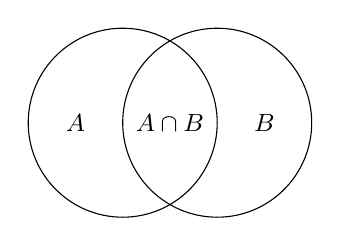
\begin{tikzpicture}[scale=0.8]

\draw (0,0) circle (1.5);
\draw (1.5,0) circle (1.5);

\node at (-0.75,0) {\small $A$};
\node at (2.25,0) {\small $B$};
\node at (0.75,0) {\small $A \cap B$};

\end{tikzpicture}
\end{center}


El nostre objectiu és calcular la mida de la unió $A \cup B$ que
correspon a l'àrea de la regió que pertany a almenys un cercle. La
imatge mostra que podem calcular l'àrea de $A \cup B$ sumant primer
les àrees de $A$ i $B$ i després restant l'àrea de $A \cap B$.

La mateixa idea es pot aplicar quan el nombre de conjunts és més
gran. Quan hi ha tres conjunts, la fórmula d'inclusió-exclusió és
\[ |A \cup B \cup C| = |A| + |B| + |C| - |A \cap B|  - |A \cap C|  - |B \cap C| + |A \cap B \cap C| \]
i la imatge corresponent és


\begin{center}
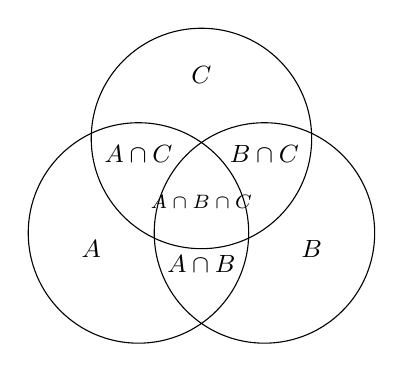
\begin{tikzpicture}[scale=0.8]

\draw (0,0) circle (1.75);
\draw (2,0) circle (1.75);
\draw (1,1.5) circle (1.75);

\node at (-0.75,-0.25) {\small $A$};
\node at (2.75,-0.25) {\small $B$};
\node at (1,2.5) {\small $C$};
\node at (1,-0.5) {\small $A \cap B$};
\node at (0,1.25) {\small $A \cap C$};
\node at (2,1.25) {\small $B \cap C$};
\node at (1,0.5) {\scriptsize $A \cap B \cap C$};

\end{tikzpicture}
\end{center}


En el cas general, la mida de la unió $X_1 \cup X_2 \cup \cdots \cup
X_n$ es pot calcular passant per totes les interseccions possibles que
contenen alguns dels conjunts $X_1,X_2,\ldots,X_n$. Si la intersecció
conté un nombre senar de conjunts, la seva mida s'afegeix a la
resposta i, en cas contrari, la seva mida es resta de la resposta.

Tingueu en compte que hi ha fórmules similars per calcular la mida
d'una intersecció a partir de les mides de les unions. Per exemple,
\[ |A \cap B| = |A| + |B| - |A \cup B|\]
i
\[ |A \cap B \cap C| = |A| + |B| + |C| - |A \cup B|  - |A \cup C|  - |B \cup C| + |A \cup B \cup C| .\]


\subsubsection{Desarranjament}

\index{Desarranjament}

Com a exemple, comptem el nombre de \key{desarranjaments}
(\emph{derangements}) dels elements $\{1,2,\ldots,n\}$, és a dir,
permutacions on cap element roman al seu lloc original. Per exemple,
quan $n=3$, hi ha dos desarranjaments: $(2,3,1)$ i $(3,1,2)$.

Una manera de resoldre el problema és utilitzar la
inclusió-exclusió. Sigui $X_k$ el conjunt de permutacions que contenen
l'element $k$ a la posició $k$. Per exemple, quan $n=3$, els conjunts
són els següents:

\[
\begin{array}{lcl}
X_1 & = & \{(1,2,3),(1,3,2)\} \\
X_2 & = & \{(1,2,3),(3,2,1)\} \\
X_3 & = & \{(1,2,3),(2,1,3)\} \\
\end{array}
\]
Amb aquests conjunts, el nombre de desarranjaments és igual
\[ n! - |X_1 \cup X_2 \cup \cdots \cup X_n|, \]
i per tant n'hi ha prou amb calcular la mida de la unió. Amb
l'inclusió-exclusió això es redueix a calcular les mides de les
interseccions, i això es pot fer de manera eficient. Per exemple, quan
$n=3$, la mida de $|X_1 \cup X_2 \cup X_3|$ és
\[
\begin{array}{lcl}
 & & |X_1| + |X_2| + |X_3| - |X_1 \cap X_2|  - |X_1 \cap X_3|  - |X_2 \cap X_3| + |X_1 \cap X_2 \cap X_3| \\
 & = & 2+2+2-1-1-1+1 \\
 & = & 4, \\
\end{array}
\]
per tant, el nombre de solucions és $3!-4=2$.

Aquest problema també es pot resoldre sense fer servir
inclusió-exclusió. Sigui $f(n)$ el nombre de desarranjaments per a
$\{1,2,\ldots,n\}$. Podem utilitzar la següent fórmula recursiva:


\begin{equation*}
    f(n) = \begin{cases}
               0               & n = 1\\
               1               & n = 2\\
               (n-1)(f(n-2) + f(n-1)) & n>2 \\
           \end{cases}
\end{equation*}


La fórmula es deriva considerant com canvia l'element 1 en un desarranjament.
Hi ha $n-1$ maneres de triar un element $x$ que substitueixi l'element 1.
En cadascuna d'aquestes eleccions, n'hi ha dues possibilitats:

\textit{Opció 1:} Substituïm l'element $x$ per l'element 1. Per
tant, la tasca restant és construir un desarranjamant de $n-2$ elements.

\textit{Opció 2:} Substituïm l'element $x$ per algun altre element que
no sigui 1.  Per tant, la tasca restant és construir un desarranjament
de $n-1$ elements, ja que no podem substituir l'element $x$ per
l'element $1$, i tots els altres elements s'han de canviar.

\section{Lema de Burnside}

\index{Lema de Burnside}

El \key{lema de Burnside} %\footnote{En realitat, Burnside no va descobrir aquest lema; només ho va esmentar al seu llibre \cite{bur97}.}
es pot utilitzar per comptar el nombre de combinacions de manera que
només es compti un representant per a cada grup de combinacions
simètriques. El lema de Burnside afirma que el nombre de combinacions
és
\[\sum_{k=1}^n \frac{c(k)}{n},\]
on hi ha $n$ maneres de canviar la posició d'una combinació, i hi ha
$c(k)$ combinacions que no canvien quan s'aplica la $k$-éssima manera de canviar
la posició d'una combinació.

Com a exemple, calculem el nombre de collarets de $n$ perles, on cada
perla té $m$ colors possibles. Dos collarets són simètrics si són
semblants després de girar-los. Per exemple, el collaret
\begin{center}
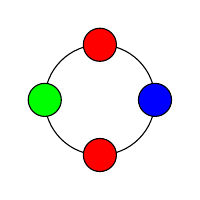
\begin{tikzpicture}[scale=0.7]
\draw[fill=white] (0,0) circle (1);
\draw[fill=red] (0,1) circle (0.3);
\draw[fill=blue] (1,0) circle (0.3);
\draw[fill=red] (0,-1) circle (0.3);
\draw[fill=green] (-1,0) circle (0.3);
\end{tikzpicture}
\end{center}
té els següents collarets simètrics:
\begin{center}
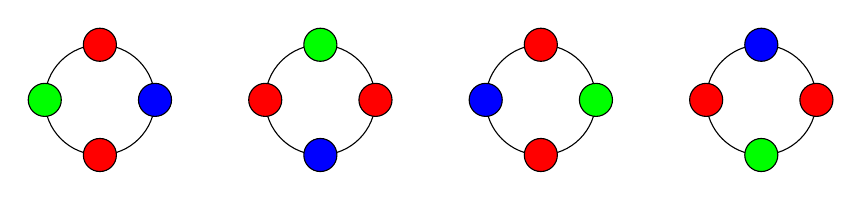
\begin{tikzpicture}[scale=0.7]
\draw[fill=white] (0,0) circle (1);
\draw[fill=red] (0,1) circle (0.3);
\draw[fill=blue] (1,0) circle (0.3);
\draw[fill=red] (0,-1) circle (0.3);
\draw[fill=green] (-1,0) circle (0.3);

\draw[fill=white] (4,0) circle (1);
\draw[fill=green] (4+0,1) circle (0.3);
\draw[fill=red] (4+1,0) circle (0.3);
\draw[fill=blue] (4+0,-1) circle (0.3);
\draw[fill=red] (4+-1,0) circle (0.3);

\draw[fill=white] (8,0) circle (1);
\draw[fill=red] (8+0,1) circle (0.3);
\draw[fill=green] (8+1,0) circle (0.3);
\draw[fill=red] (8+0,-1) circle (0.3);
\draw[fill=blue] (8+-1,0) circle (0.3);

\draw[fill=white] (12,0) circle (1);
\draw[fill=blue] (12+0,1) circle (0.3);
\draw[fill=red] (12+1,0) circle (0.3);
\draw[fill=green] (12+0,-1) circle (0.3);
\draw[fill=red] (12+-1,0) circle (0.3);
\end{tikzpicture}
\end{center}
Hi ha $n$ maneres de canviar la posició d'un collaret, perquè el podem
girar $0,1,\ldots,n-1$ passos en sentit horari. Si el nombre de passos
és 0, tots els $m^n$ collarets romanen iguals, i si el nombre de
passos és 1, només els $m$ collarets on cada perla té el mateix color
romandran iguals.

De manera més general, quan el nombre de passos és $k$, un total de
\[m^{\textrm{gcd}(k,n)}\]
collarets segueixen sent els mateixos, on $\textrm{gcd}(k,n)$ és
el màxim comú divisor de $k$ i $n$. La raó d'això és que els blocs de
perles de mida $\textrm{gcd}(k,n)$ es substituiran mútuament. Així,
segons el lema de Burnside, el nombre de collarets és

\[\sum_{i=0}^{n-1} \frac{m^{\textrm{gcd}(i,n)}}{n}. \]
Per exemple, el nombre de collarets de longitud 4 amb 3 colors és
\[\frac{3^4+3+3^2+3}{4} = 24. \]


\section{Fórmula de Cayley}

\index{Fórmula de Cayley}
\label{cayley-formula}

\key{Fórmula de Cayley} % \footnote{Si bé la fórmula porta el nom d'A. Cayley, % que la va estudiar el 1889, va ser descoberta abans per CW Borchardt el 1860.}
afirma que hi ha $n^{n-2}$ arbres etiquetats amb $n$
nodes. Els nodes s'etiqueten $1,2,\ldots,n$, i dos arbres són
diferents si la seva estructura o l'etiquetatge és diferent.


\begin{samepage}
For example, when $n=4$, the number of labeled
trees is $4^{4-2}=16$:

\begin{center}
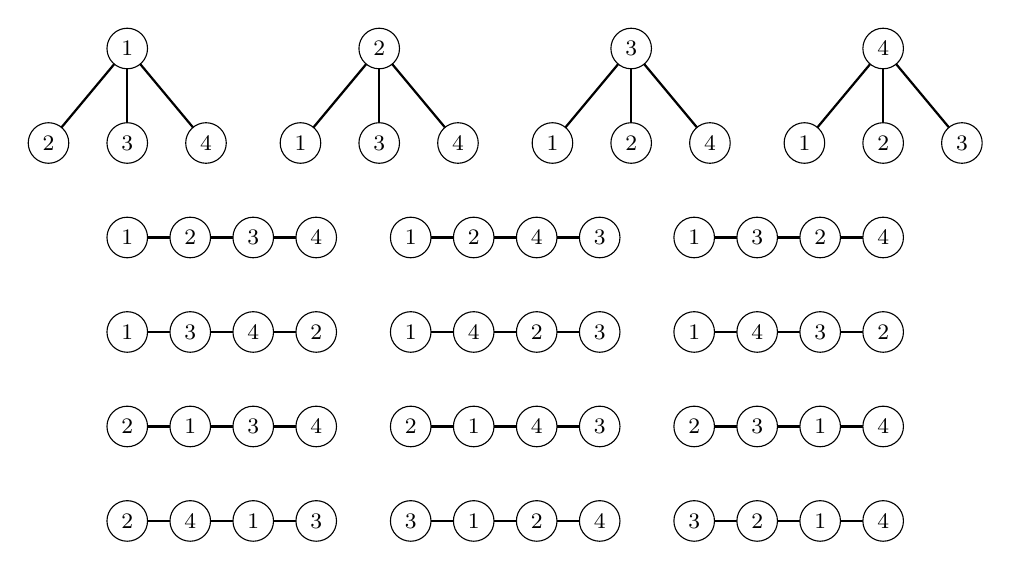
\begin{tikzpicture}[scale=0.8]
\footnotesize

\newcommand\puua[6]{
\path[draw,thick,-] (#1,#2) -- (#1-1.25,#2-1.5);
\path[draw,thick,-] (#1,#2) -- (#1,#2-1.5);
\path[draw,thick,-] (#1,#2) -- (#1+1.25,#2-1.5);
\node[draw, circle, fill=white] at (#1,#2) {#3};
\node[draw, circle, fill=white] at (#1-1.25,#2-1.5) {#4};
\node[draw, circle, fill=white] at (#1,#2-1.5) {#5};
\node[draw, circle, fill=white] at (#1+1.25,#2-1.5) {#6};
}
\newcommand\puub[6]{
\path[draw,thick,-] (#1,#2) -- (#1+1,#2);
\path[draw,thick,-] (#1+1,#2) -- (#1+2,#2);
\path[draw,thick,-] (#1+2,#2) -- (#1+3,#2);
\node[draw, circle, fill=white] at (#1,#2) {#3};
\node[draw, circle, fill=white] at (#1+1,#2) {#4};
\node[draw, circle, fill=white] at (#1+2,#2) {#5};
\node[draw, circle, fill=white] at (#1+3,#2) {#6};
}

\puua{0}{0}{1}{2}{3}{4}
\puua{4}{0}{2}{1}{3}{4}
\puua{8}{0}{3}{1}{2}{4}
\puua{12}{0}{4}{1}{2}{3}

\puub{0}{-3}{1}{2}{3}{4}
\puub{4.5}{-3}{1}{2}{4}{3}
\puub{9}{-3}{1}{3}{2}{4}
\puub{0}{-4.5}{1}{3}{4}{2}
\puub{4.5}{-4.5}{1}{4}{2}{3}
\puub{9}{-4.5}{1}{4}{3}{2}
\puub{0}{-6}{2}{1}{3}{4}
\puub{4.5}{-6}{2}{1}{4}{3}
\puub{9}{-6}{2}{3}{1}{4}
\puub{0}{-7.5}{2}{4}{1}{3}
\puub{4.5}{-7.5}{3}{1}{2}{4}
\puub{9}{-7.5}{3}{2}{1}{4}
\end{tikzpicture}
\end{center}
\end{samepage}


A continuació veurem com es pot derivar la fórmula de Cayley
mitjançant els codis de Prüfer.

\subsubsection{Codi Prüfer}

\index{Codi Prüfer}

Un \key{codi Prüfer} %\footnote{L'any 1918, H. Prüfer va demostrar el teorema de Cayley utilitzant els codis de Prüfer \cite{pru18}.}
és una seqüència de $n-2$ nombres que descriu un arbre etiquetat. La codificació es
construeix seguint un procés que elimina $n-2$ fulles de l'arbre. A
cada pas, s'elimina la fulla amb l'etiqueta més petita i s'afegeix a la codificació
l'etiqueta del seu únic veí.

Per exemple, calculem el codi Prüfer del graf següent:
\begin{center}
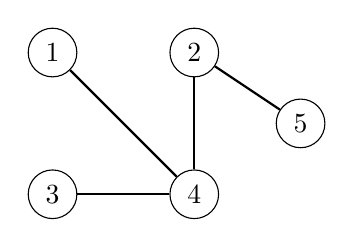
\begin{tikzpicture}[scale=0.9]
\node[draw, circle] (1) at (2,3) {$1$};
\node[draw, circle] (2) at (4,3) {$2$};
\node[draw, circle] (3) at (2,1) {$3$};
\node[draw, circle] (4) at (4,1) {$4$};
\node[draw, circle] (5) at (5.5,2) {$5$};

\path[draw,thick,-] (1) -- (4);
\path[draw,thick,-] (3) -- (4);
\path[draw,thick,-] (2) -- (4);
\path[draw,thick,-] (2) -- (5);
\end{tikzpicture}
\end{center}


Primer eliminem el node 1 i afegim el node 4:
\begin{center}
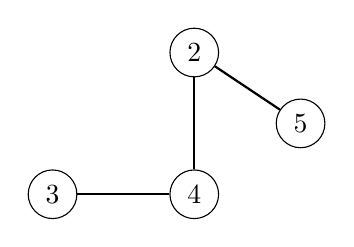
\begin{tikzpicture}[scale=0.9]
%\node[draw, circle] (1) at (2,3) {$1$};
\node[draw, circle] (2) at (4,3) {$2$};
\node[draw, circle] (3) at (2,1) {$3$};
\node[draw, circle] (4) at (4,1) {$4$};
\node[draw, circle] (5) at (5.5,2) {$5$};

%\path[draw,thick,-] (1) -- (4);
\path[draw,thick,-] (3) -- (4);
\path[draw,thick,-] (2) -- (4);
\path[draw,thick,-] (2) -- (5);
\end{tikzpicture}
\end{center}


A continuació, eliminem el node 3 i afegim el node 4:
\begin{center}
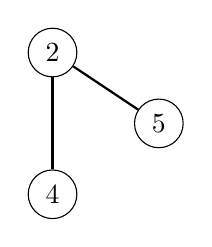
\begin{tikzpicture}[scale=0.9]
%\node[draw, circle] (1) at (2,3) {$1$};
\node[draw, circle] (2) at (4,3) {$2$};
%\node[draw, circle] (3) at (2,1) {$3$};
\node[draw, circle] (4) at (4,1) {$4$};
\node[draw, circle] (5) at (5.5,2) {$5$};

%\path[draw,thick,-] (1) -- (4);
%\path[draw,thick,-] (3) -- (4);
\path[draw,thick,-] (2) -- (4);
\path[draw,thick,-] (2) -- (5);
\end{tikzpicture}
\end{center}


Finalment eliminem el node 4 i afegim el node 2:
\begin{center}
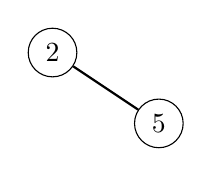
\begin{tikzpicture}[scale=0.9]
%\node[draw, circle] (1) at (2,3) {$1$};
\node[draw, circle] (2) at (4,3) {$2$};
%\node[draw, circle] (3) at (2,1) {$3$};
%\node[draw, circle] (4) at (4,1) {$4$};
\node[draw, circle] (5) at (5.5,2) {$5$};

%\path[draw,thick,-] (1) -- (4);
%\path[draw,thick,-] (3) -- (4);
%\path[draw,thick,-] (2) -- (4);
\path[draw,thick,-] (2) -- (5);
\end{tikzpicture}
\end{center}


Així, el codi Prüfer del graf és $[4,4,2]$.

Podem construir un codi Prüfer per a qualsevol arbre, i el que és més
important, l'arbre original es pot reconstruir a partir d'un codi
Prüfer. Per tant, el nombre d'arbres etiquetats de $n$ nodes és igual
a $n^{n-2}$, que és el nombre de codis Prüfer de mida $n$.
